\chapter{Evaluation}\label{sec:eval}

Im folgenden wird der Gebrauch von Rust im Zusammenhang mit dem invasiven Computing evaluiert. Hierbei
wird vor allem mit den bereits unterstützten Sprachen C und X10 verglichen.

\section{Laufzeitverhalten und Dateigröße}

Zu Beginn werden

\subsection{Vergleich der Anlaufzeit}

Es wird überprüft, wie lange ein Programm, welches in einer der respektiven Programmiersprachen geschrieben wurde,
benötigt, um zu starten und anschließend sofort wieder aufzuhören.

Startup %TODO Screenshot startup 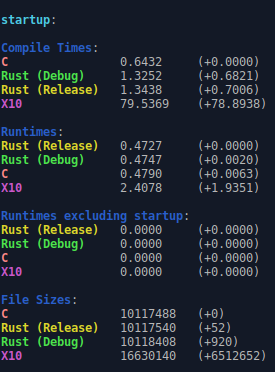
\includegraphics{eval-screenshots/startup.jpg}  

Auswertung %TODO Auswerten

\subsection{Berechnen von Primzahlen}

Um die Rechenleistung der verschiedenen Programmiersprachen bei einem intensiveren Problem zu vergleichen, wurden
Programme geschrieben welche Primzahlen berechnen. Hierbei wurden zwei unterschiedliche Ansätze verwendet: Zum einen
eine naive Berechnung welche jede Zahl individuell auf Teilbarkeit mit kleineren Zahlen prüft und andererseits
das Sieb von Eratosthenes, eine effiziente Methode zum Berechnen von Primzahlen.

Naiv %TODO Naive Prime \includegraphics{eval-screenshots/naive-prime.jpg}

Eratosthenes %TODO eratosthenes  \includegraphics{eval-screenshots/eratosthenes-prime.jpg}

Auswertung %TODO Auswerten


\subsection{Müll-Ersteller}

X10 verwaltet den Speicher mithilfe eines Garbage Collectors, wobei C und Rust ohne einen solchen auskommen.
In C muss jedoch 

GarbageOnly  %TODO garbage  \includegraphics{eval-screenshots/garbage.jpg}


\section{Sicherheit}

Im folgenden wird die Sicherheit bezüglich undefiniertem Verhalten als Folge von fehlerhaften Speicherzugriffen analysiert.
Hierbei ist vor allem der Vergleich zwischen Rust und C interessant, da einige von Rusts primären Eigenschaften 

\subsection{Undefiniertes Verhalten}

Undefiniertes Verhalten (Wird in rust vom Kompiler verhindert)


\section{Abstraktionen}

Es werden nun die implementierten Abstraktionen der octolib Bibliothek mit den Implementierungen in C und X10 verglichen.

\section{Minimales Infect}

\section{Cleanup}

\section{Closures}


